\documentclass[11pt]{article}
\usepackage{geometry}                % See geometry.pdf to learn the layout options. There are lots.
\geometry{letterpaper}                   % ... or a4paper or a5paper or ... 
%\geometry{landscape}                % Activate for for rotated page geometry
%\usepackage[parfill]{parskip}    % Activate to begin paragraphs with an empty line rather than an indent
\usepackage{graphicx}
\usepackage{amssymb,amsmath}
\usepackage{epstopdf}
\usepackage{pgf}
\usepackage{pgfpages}
\usepackage{tikz}
\usetikzlibrary{arrows,backgrounds}
\usepgflibrary{shapes}
\DeclareGraphicsRule{.tif}{png}{.png}{`convert #1 `dirname #1`/`basename #1 .tif`.png}
\pagestyle{empty}


\begin{document}
 \begin{center}
   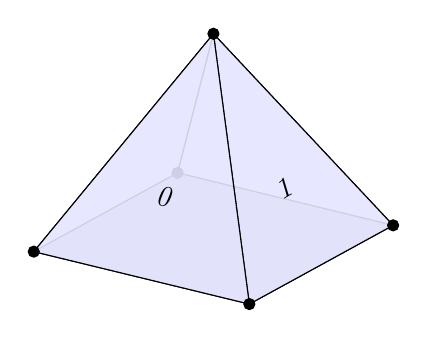
\begin{tikzpicture}[join=round] % Pyramid Faces
       \filldraw[fill=blue!10,fill opacity=0.4](0,2.6)--(-2.282,-.167)--(-.456,.833)--(0,2.6)--cycle;
       \filldraw[fill=blue!10,fill opacity=0.4](0,2.6)--(-.456,.833)--(2.282,.167)--(0,2.6)--cycle;
       \filldraw[fill=black!20](2.282,.167)--(-.456,.833)--(-2.282,-.167)--(.456,-.833)--cycle;
       \filldraw(-.456,.833) circle (2pt);
       \filldraw[fill=blue!10,fill opacity=0.9](0,2.6)--(2.282,.167)--(.456,-.833)--(0,2.6)--cycle;
       \filldraw[fill=blue!10,fill opacity=0.9](0,2.6)--(.456,-.833)--(-2.282,-.167)--(0,2.6)--cycle;
       \filldraw(2.282,.167) circle (2pt);
       \filldraw(-2.282,-.167) circle (2pt);
       \filldraw(0,2.6) circle (2pt);
       \filldraw(.456,-.833) circle (2pt);
       \fill[black]
                (-.609,.533) node [xslant=.4,yslant=-0.2] {0}
                (.913,.644) node [xslant=-.3,yslant=.5] {1};
   \end{tikzpicture}
  \hspace{1cm}
   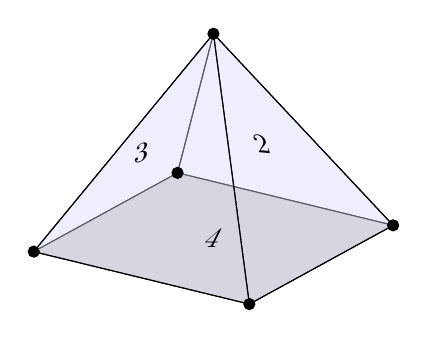
\begin{tikzpicture}[join=round] % Pyramid Faces
       \filldraw[fill=blue!10,fill opacity=0.4](0,2.6)--(-2.282,-.167)--(-.456,.833)--(0,2.6)--cycle;
       \filldraw[fill=blue!10,fill opacity=0.4](0,2.6)--(-.456,.833)--(2.282,.167)--(0,2.6)--cycle;
       \filldraw[fill=black!20](2.282,.167)--(-.456,.833)--(-2.282,-.167)--(.456,-.833)--cycle;
       \filldraw[fill=blue!10,fill opacity=0.4](0,2.6)--(2.282,.167)--(.456,-.833)--(0,2.6)--cycle;
       \filldraw[fill=blue!10,fill opacity=0.4](0,2.6)--(.456,-.833)--(-2.282,-.167)--(0,2.6)--cycle;
       \filldraw(-.456,.833) circle (2pt);
       \filldraw(2.282,.167) circle (2pt);
       \filldraw(-2.282,-.167) circle (2pt);
       \filldraw(0,2.6) circle (2pt);
       \filldraw(.456,-.833) circle (2pt);
       \fill[black]
                (.609,1.2) node [xslant=-0.4,yslant=-.1] {2}
                (-.913,1.089) node [xslant=.1,yslant=.4] {3}
                (0,0) node [xslant=.5] {4};
   \end{tikzpicture}
 \end{center}
\end{document}  
